%Este trabalho está licenciado sob a Licença Atribuição-CompartilhaIgual 4.0 Internacional Creative Commons. Para visualizar uma cópia desta licença, visite http://creativecommons.org/licenses/by-sa/4.0/deed.pt_BR ou mande uma carta para Creative Commons, PO Box 1866, Mountain View, CA 94042, USA.

\chapter{Outros sistemas de coordenadas}\label{cap_osc}
\thispagestyle{fancy}

Neste capítulo, vamos introduzir outros sistemas de coordenadas no plano e no espaço tridimensional.

\section{Sistema de coordenadas polares}\label{cap_osc_scp}

No plano, o sistema de coordenadas polares é definido por um ponto de origem (cahamdo de \emph{polo}) e um eixo orientado $Ox$ (chamado de \emph{eixo polar}). Veja a Figura \ref{fig:osc_scp}.

\begin{figure}[H]
  \centering
  \includegraphics[width=0.6\textwidth]{cap_osc/dados/fig_osc_scp/fig}
  \caption{Sistema de coordenadas polares.}
  \label{fig:osc_scp}
\end{figure}

Neste sistema, um ponto $P$ de coordenadas polares ${\color{blue}P=(r, \theta)}$ é tal que ${\color{blue}|OP| = r}$ (i.e. a distância do polo ao ponto é $r$) e ${\color{blue}\theta}$ é o ângulo de $Ox$ com $OP$, medido positivamente no sentido anti-horário.

\begin{ex}
  Na Figura \ref{fig:ex_osc_scp}, temos a representação dos pontos ${\color{blue}P=(2\sqrt{2}, \frac{\pi}{4})}$, ${\color{red}A=(2, \frac{2\pi}{3})}$ e ${\color{orange}B=(\sqrt{2}, \frac{5\pi}{4})}$ no sistema de coordenadas polares.

\begin{figure}[H]
  \centering
  \includegraphics[width=0.6\textwidth]{cap_osc/dados/fig_ex_osc_scp/fig}
  \caption{Sistema de coordenadas polares.}
  \label{fig:ex_osc_scp}
\end{figure}  
\end{ex}

\begin{obs}
  Por convenção, as coordenadas polares $(r, \pi + \theta) = (-r, \theta)$, $r>0$. Por exemplo, $B=(\sqrt{2}, \frac{5\pi}{4}) = (-\sqrt{2}, \frac{\pi}{4})$. Veja na Figura \ref{fig:ex_osc_scp}.
\end{obs}

\subsection{Coordenadas cartesianas x polares}

Aqui, vamos estudar como podemos converter as coordenadas de um ponto $P$ de coordenadas cartesianas para coordenadas polares e vice-e-versa. Vamos denotar as coordenadas cartesianas do ponto $P$ por $P=(x_P, y_P)$ e suas coordenadas polares por $P=(r, \theta)$. Veja a Figura \ref{fig:osc_ccxcp}.

\begin{figure}[H]
  \centering
  \includegraphics[width=0.5\textwidth]{cap_osc/dados/fig_osc_ccxcp/fig}
  \caption{Sistema de coordenadas polares.}
  \label{fig:osc_ccxcp}
\end{figure}  

Na Figura \ref{fig:osc_ccxcp}, vamos nos concentrar no triângulo retângulo de vértices $O$, $(x_P, 0)$ e $P$. Das relações trigonométricas e do teorema de Pitágoras, temos que
\begin{gather}
  \cos\theta = \frac{x_P}{r} \\
  \sen\theta = \frac{y_P}{r} \\
  r^2 = x_P^2 + y_P^2 \\
  \tg\theta = \frac{y_P}{x_P}
\end{gather}
ou, equivalentemente,
\begin{gather}
  {\color{blue}x_P = r\cos\theta} \\
  {\color{blue}y_P = r\sen\theta} \\
  {\color{blue}r = \sqrt{x_P^2 + y_P^2 }} \\
  {\color{blue}\theta = \arc\tg\left(\frac{y_P}{x_P}\right)}
\end{gather}

\begin{ex}
  \emconstrucao
\end{ex}

\emconstrucao

\subsection{Exercícios resolvidos}

\emconstrucao

\subsection*{Exercícios}

\emconstrucao